\documentclass[12pt,letterpaper]{article}

%Note to Self:
%When Decommission? - after two months of feeling useless or right away?

\usepackage[utf8]{inputenc}
\usepackage[letterpaper,margin=1in]{geometry}
\usepackage{caption} % for table captions

\usepackage{amsmath} % for multi-line equations and piecewises
\usepackage{indentfirst} % to indent after a section
\usepackage{setspace}
\usepackage{times}
\usepackage{graphicx}
\usepackage{textcomp}
\usepackage{xspace}
\usepackage{verbatim} % for block comments
\usepackage{subfig} % for subfigures
\usepackage{enumitem} % for a) b) c) lists
\usepackage{tabularx}
\usepackage{cleveref}
\usepackage{xcolor}
\usepackage{soul}
\newcommand{\mathcolorbox}[2]{\colorbox{#1}{$\displaystyle #2$}}

\newcolumntype{b}{X}
\newcolumntype{s}{>{\hsize=.5\hsize}X}
\newcolumntype{m}{>{\hsize=.75\hsize}X}
\usepackage{titling}
\usepackage{minted}

\newcommand{\subtitle}[1]{%
  \posttitle{%
    \par\end{center}
    \begin{center}\large#1\end{center}
    \vskip0.5em}%
}
\usepackage{tikz}


\usetikzlibrary{shapes.geometric,arrows}
\tikzstyle{process} = [rectangle, rounded corners, minimum width=3cm, minimum height=1cm,text centered, draw=black, fill=blue!30]
\tikzstyle{arrow} = [thick,->,>=stealth]


\graphicspath{{images/}}
 
\usepackage[font={footnotesize,it}]{caption}
 



\setlength{\parindent}{15pt} % Default is 15pt.




\fontfamily{ptm}\selectfont

\title{CP1 for NPRE 501}
\author{Jin Whan Bae}
\date{2017-11-01}


\begin{document}
	
	\maketitle
	\hrule
	\onehalfspacing
	\thispagestyle{empty}

\section{Problem Definition}

\Cref{tab:constants} lists the constants used in the problem.


\begin{table}[h]
     \centering
    \begin{tabularx}{\textwidth}{bbb}
       \hline
       Parameter & Value & [Unit] \\
       \hline
       Diamater & 6 & [cm] \\
       \textbf{Radius} & \textbf{3} & [cm] \\
       Geometry & Sphere \\
       k & 15 & [$ \frac{W}{mK} $] \\
       Density & 8000 & [$ \frac{kg}{m^3} $] \\
       Specific Heat & 500 & [$ \frac{J}{kgK} $] \\
       \textbf{$ \alpha$} & \textbf{3.75e-6} & [$ \frac{m^2}{s} $] \\
       \hline
    \end{tabularx}
    \caption {Problem Constants. Derived constants are in bold.}
    \label{tab:constants}
\end{table}

Differential Equation:
\[\frac{1}{\alpha} \cdot \frac{dT}{dt} = \frac{1}{r^2} \frac{d}{dr} r^2 \frac{dT}{dr}\]

Boundary Conditions:
\[T(0,t) = finite \quad OR \quad \frac{dT}{dr} (r = 0, t) = 0\]
\[\frac{dT}{dr} (r = R) = 0 \]

Initial Condition:
\[T(r,0) = \frac{T_0}{2} (1-\cos{(\frac{\pi \cdot r}{R})}) \]


\subsection{Finding Steady State}
Since there is no heat generation or leakage (r=R is insulated), 
the steady state temperature is a constant throughout the sphere.

Expressing mathematically,

$T_{ss}$ is when $\frac{dT}{dt} = 0 $:

\[0 = \frac{1}{r^2} \frac{d}{dr} r^2 (\frac{dT_{ss}}{dr})\]

\[\frac{C_1}{r^2} = \frac{dT_{ss}}{dr}\]

\[-\frac{C_1}{r} + C_2 = T_{ss}\]

applying BC:

at r = 0, finite, makes  $C_1 = 0$

\[T_{ss} = C_2\]

the numerical value of this constant can be found doing an energy balance
of the system.

\[\int_{0}^{R} \frac{T_0}{2} (1-\cos(\frac{\pi r}{R})) r^2 dr = \int_{0}^{R} C r^2 dr \]

\[\frac{T_0}{2} \int_{0}^{R}  (r^2-r^2\cos(\frac{\pi r}{R})) dr = C \frac{R^3}{3} \]

using separation of variables:

\[\frac{T_0}{2} ( \frac{R^3}{3} - (\frac{r^2 R}{\pi} \sin(\frac{\pi r}{R})\Big|_0^R - \frac{2R}{\pi} \int_0^R r \sin(\frac{\pi r}{R})))dr = C \frac{R^3}{3}\]

Solving this:

\[\frac{T_0}{2} (\frac{R^3}{3} + \frac{2R^3}{\pi ^2}) = C \frac{R^3}{3} \]

\centering{
    \mathcolorbox{yellow}{
    C = T_{ss} = \frac{3T_0}{2} (\frac{\pi^2 + 6}{3\pi^2}) \approx 0.804 T_0
}


\section{Numerical Solution}


\[\frac{1}{\alpha} \cdot \frac{dT}{dt} = \frac{2}{r} \frac{dT}{dr} + \frac{d^2T}{dr^2}\]

Applying the finite difference method, central for r and explicit for t:
\[\frac{1}{\alpha} \cdot \frac{T_k^{u} - T_k^{u-1}}{\Delta t} = \frac{2}{r_k} \; (\frac{T^{u-1}_{k+1}-T^{u-1}_{k-1}}{2 \Delta r}) + \frac{T^{u-1}_{k-1} - 2T^{u-1}_k + T^{u-1}_{k+1}}{\Delta r^2}\]

where u is the temporal step and k is the spacial step.

Solving for $T_{k}^{u+1}$:

\centering{
    \mathcolorbox{yellow}{
    T_{k}^{u+1} = T_k^u + \alpha \frac{\Delta t }{\Delta r \cdot r} (T_{k+1}^u + T_{k-1}^u) + \alpha * \frac{\Delta t}{(\Delta r)^2} (T_{k+1}^{u} -2T_k^u + T_{k-1}^u) }
}


Applying neuman boundary condition at r=0:
\[\frac{dT(0,t)}{dr} =0 \]
\[\frac{T_1^u - T_{-1}^u}{2\Delta r} =0 \]
\[T_1^u = T_{-1}^u\]

This gives:

\centering{
    \mathcolorbox{yellow}{T_0^{u+1} = T_0^u + \alpha * \frac{\Delta t}{(\Delta r)^2} (2T_{1}^{u} -2T_0^u ) }
}


Applying neuman boundary condition at r=R (k=K at r=R):
\[-k \frac{dT(R,t)}{dr} =0 \]
\[\frac{T_{K+1}^u - T_{K-1}^u}{2\Delta r} =0 \]
\[T_{K+1}^u = T_{K-1}^u\]

This gives:

\centering{
    \mathcolorbox{yellow}{T_K^{u+1} = T_K^u + \alpha * \frac{\Delta t}{(\Delta r)^2} (2T_{K-1}^{u} -2T_K^u )}
}

\section{Appendix A}

\subsection{a. Final Temperature Distribution in the Sphere}
The final temperature distribution will be a cosine curve
with the highest point at r = 0, gradually going down to
the minimum value at r = R. 

\section{Appendix B}

\subsection{Analytical solution for solving T(r,t) directly}

\[\frac{1}{\alpha} \cdot \frac{dT}{dt} = \frac{1}{r^2} \frac{d}{dr} r^2 \frac{dT}{dr}\]

Boundary Conditions:
\[T(0,t) = finite \]
\[\frac{dT}{dr} (r = R) = 0 \]

Initial Condition:
\[T(r,0) = \frac{T_0}{2} (1-\cos{(\frac{\pi \cdot r}{R})}) \]

set:
\[T(r,t) = \frac{\overline{T} (r,t)}{r} +T_ss\]
\[\overline{T} (r,t) = T(r,t) r + T_ss r\]

plugging this back into the differential equation:

\[\frac{1}{\alpha} \cdot \frac{d\overline{T}}{dt} \frac{1}{r} = \frac{1}{r^2} \frac{d}{dr} r^2 (\frac{d\overline{T}}{dr} \frac{1}{r} - \frac{1}{r^2} \overline{T}) \]

\[\frac{1}{\alpha} \cdot \frac{d\overline{T}}{dt} = \frac{1}{r} \frac{d}{dr} (\frac{d\overline{T}}{dr} r - \overline{T}) \]

\[\frac{1}{\alpha} \cdot \frac{d\overline{T}}{dt} = \frac{1}{r} (\frac{d^2\overline{T}}{dr^2} r + \frac{d\overline{T}}{dr} - \frac{d\overline{T}}{dr}) \]

\[\frac{1}{\alpha} \cdot \frac{d\overline{T}}{dt} = \frac{d^2\overline{T}}{dr^2} \]

where 
\[\overline{T}(0,t) = 0 \]
\[\frac{d\overline{T}}{dr} = \frac{\overline{T}}{R}\]
and initial condition
\[\overline{T} (r,0) = r \frac{T_0}{2} (1- cos(\frac{\pi r}{R})) - T_{ss} r\]

This turns into a cartesian problem.

Applying Separation of Variables:
\[\overline{T}(r,t) = \Gamma (t) \Psi (r)  \]

Applying the new variables, dividing both sides by $\Gamma (t) \Psi (r) $,
and setting it to a new variable $ -\beta^2 $:
\[\frac{1}{\alpha  \Gamma} \cdot \frac{d\Gamma}{dt} = \frac{d^2 \Psi}{dr^2} \frac{1}{\Psi} = -\beta^2 \] 

Solving for $\Psi$ first:
\[\frac{d^2 \Psi}{dr^2} \frac{1}{\Psi} = -\beta^2 \]

\[\frac{d^2 \Psi}{dr^2} + \beta^2 \Psi = 0 \]

\[\Psi (r) = C_1 sin(\beta r) + C_2 cos(\beta r) \]

Boundary Conditions:

Since:
\[\frac{dT}{dr} = -\frac{\overline{T}}{r^2} + \frac{1}{r} \frac{d\overline{T}}{dr}\]

The boundary conditions become:
\[-\Psi(r=0) = 0 \]
\[-k (\frac{\Psi}{R^2} + \frac{d\Psi}{dr} \frac{1}{R}) = 0  \]

Applying the first boundary condition,
interpreting as $\Psi(r=0) = 0 , C_2 = 0$

Applying the second boundary condition,
\[-\frac{C_1 \sin(\beta R)}{R^2} + C_1 \cos(\beta r) \beta = 0 \]
\[-\sin(\beta R) + R \beta \cos{\beta R} =0 \]
\[\tan(\beta R ) = R\beta \]


\begin{figure}[htbp!]
  \begin{center}
    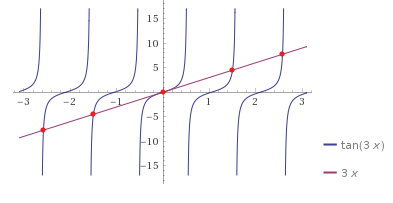
\includegraphics[scale=0.7]{tan_plot.png}
  \end{center}
  \caption{Plot of tan(3x) = 3x.}
  \label{fig:tan_plot}
\end{figure}

$\beta$ is the zeros of that equation (illustrated in \cref{fig:tan_plot})

Solving for $\Gamma(t)$:
\[\frac{1}{\alpha  \Gamma} \cdot \frac{d\Gamma}{dt} = -\beta_n^2 \]
\[\frac{1}{\alpha  \Gamma} \cdot \frac{d\Gamma}{dt} = -\beta_n^2 \alpha \Gamma \]

\[\Gamma(t) = A_1 e^{-\alpha \beta_n^2 t }\]

This makes $\overline{T}(r,t)$:

\centering{
    \mathcolorbox{yellow}{
\overline{T}(r,t) = \sum_{n=1}^{\infty} A_n e^{-\alpha \beta_n^2 t} sin(\beta_n r)
}


Applying initial condition and orthogonality:
\[T\sum_{n=1}^{\infty} A_n \sin(\beta_n r) = r \frac{T_0}{2} (1-\cos(\frac{\pi r}{R})) - T_{ss} r\]

\centering{
  \mathcolorbox{yellow}{
  A_n = \frac{\int_{0}^{R} (r \frac{T_0}{2} (1- \cos(\frac{\pi r}{R})) - T_{ss}r) \sin(\beta_n r) dr }
              {\int_{0}^{R} (\sin(\beta_n r))^2 dr}
  }
}

Plugging all this into $T(r,t)$:

\centering{
  \mathcolorbox{yellow}{
T(r,t) = \sum_{n=1}^{\infty} A_n \frac{\sin(\beta_n r)}{r} e^{-\beta_n^2 \alpha t} + T_{ss}
  }
}



\subsection{Analytical solution by defining new temperature}

\[T'(r,t) = T(r,t) - T_{ss}\]

\[T'(r,t) + T_{ss} = T(r,t) \]


where $T_{ss}$ is:


\[0 = \frac{1}{r^2} \frac{d}{dr} r^2 (\frac{dT_{ss}}{dr})\]

\[\frac{C_1}{r^2} = \frac{dT_{ss}}{dr}\]

\[-\frac{C_1}{r} + C_2 = T_{ss}\]

applying BC:

at r = 0, finite, makes  $C_1 = 0$

\[T_{ss} = C_2\]

Plugging the new definition into the original differential equation:

differential equation becomes:

\[\frac{1}{\alpha} (\frac{dT'}{dt} + \frac{dT_{ss}}{dt}) = \frac{1}{r^2} \frac{d}{dr} r^2 (\frac{dT'}{dr} + \frac{dT_{ss}}{dr})\]

Considering $\frac{dT_{ss}}{dt} = \frac{dT_{ss}}{dr} = 0$,

\[\frac{1}{\alpha} \cdot \frac{dT'}{dt} = \frac{1}{r^2} \frac{d}{dr} r^2 \cdot \frac{dT'}{dr} \]

Boundary Conditions:
\[T'(0,t)  = finite \]
\[\frac{dT'}{dr} (r = R) = 0 \]

Initial Condition:
\[T'(r,0) = \frac{T_0}{2} (1-\cos{(\frac{\pi \cdot r}{R})}) - C_2 \]

set:
\[T'(r,t) = \frac{\overline{T'}}{r} \]


\[\frac{1}{\alpha} \cdot \frac{d\overline{T'}}{dt} \frac{1}{r} = \frac{1}{r^2} \frac{d}{dr} r^2 (\frac{d\overline{T'}}{dr} \frac{1}{r} - \frac{1}{r^2} \overline{T'}) \]

\[\frac{1}{\alpha} \cdot \frac{d\overline{T'}}{dt} = \frac{1}{r} \frac{d}{dr} (\frac{d\overline{T'}}{dr} r - \overline{T'}) \]

\[\frac{1}{\alpha} \cdot \frac{d\overline{T'}}{dt} = \frac{1}{r} (\frac{d^2\overline{T'}}{dr^2} r + \frac{d\overline{T'}}{dr} - \frac{d\overline{T'}}{dr}) \]

\[\frac{1}{\alpha} \cdot \frac{d\overline{T'}}{dt} = \frac{d^2\overline{T'}}{dr^2} \]

turns into a cartesian problem.

Applying Separation of Variables:
\[\overline{T'}(r,t) = \Gamma (t) \Psi (r)  \]

Boundary Conditions:

\[\Psi(r = 0) = finite \]
\[\frac{d\Psi}{dr} (r = R) = 0 \]

Applying the new variables, dividing both sides by $\Gamma (t) \Psi (r) $,
and setting it to a new variable $ -\beta^2 $:
\[\frac{1}{\alpha  \Gamma} \cdot \frac{d\Gamma}{dt} = \frac{d^2 \Psi}{dr^2} \frac{1}{\Psi} = -\beta^2 \] 

Solving for $\Psi$ first:
\[\frac{d^2 \Psi}{dr^2} \frac{1}{\Psi} = -\beta^2 \]

\[\frac{d^2 \Psi}{dr^2} + \beta^2 \Psi = 0 \]

\[\Psi (r) = C_1 sin(\beta r) + C_2 cos(\beta r) \]

Applying the first boundary condition,
interpreting as $\Psi(r=0) = 0 , C_2 = 0$

Applying the second boundary condition,
\[-\frac{C_1 \sin(\beta R)}{R^2} + C_1 \cos(\beta r) \beta = 0 \]
\[-\sin(\beta R) + R \beta \cos{\beta R} =0 \]
\[\tan(\beta R ) = R\beta \]

$\beta$ is the zeros of that equation.

Solving for $\Gamma(t)$:
\[\frac{1}{\alpha  \Gamma} \cdot \frac{d\Gamma}{dt} = -\beta_n^2 \]
\[\frac{1}{\alpha  \Gamma} \cdot \frac{d\Gamma}{dt} = -\beta_n^2 \alpha \Gamma \]

\[\Gamma(t) = A_1 e^{-\alpha \beta_n^2 t }\]

This makes $\overline{T'}(r,t)$:
\[\overline{T'}(r,t) = A_n e^{-\alpha \beta_n^2 t} sin(\beta_n r)\]

Solving back for $T'(r,t)$:
\[T'(r,t) = \frac{A_n}{r} e^{-\alpha \beta_n^2 t} sin(\beta_n r)\]

Applying initial condition and orthogonality:
\[T'(r,0) = \frac{A_n}{r} sin(\beta_n r) = \frac{T_0}{2} (1-\cos{(\frac{\pi \cdot r}{R})}) + C_2\]

\[A_n = \frac{\int_{0}^{R}  r^3 sin(\beta_n r) (\frac{T_0}{2} \cdot (1-\cos{\frac{\pi r}{R}}) + C_2) dr} {\int_{0}^{R} r^2 \sin^2{\beta_n r} dr }\]

The analytical solution is:
\[T'(r,t) = \frac{\int_{0}^{R}  r^3 sin(\beta_n r) (\frac{T_0}{2} \cdot (1-\cos{\frac{\pi r}{R}}) + T_{ss}) dr} {\int_{0}^{R} r^2 \sin^2{\beta_n r} dr } e^{-\alpha \beta_n^2 t} sin(\beta_n r)\]

\[T = \frac{\int_{0}^{R}  r^3 sin(\beta_n r) (\frac{T_0}{2} \cdot (1-\cos{\frac{\pi r}{R}}) + T_{ss}) dr} {\int_{0}^{R} r^2 \sin^2{\beta_n r} dr } e^{-\alpha \beta_n^2 t} sin(\beta_n r) + T_{ss} \]

Since the solution from section 4.1 with $n=0$ covers the 
steady state case, this problem is redundant and provides
no new insight into the problem from section 4.1.


\subsection{Code1}
\begin{minted}{xml}
<institution>
      <name>NO_ddd</name>
       <config><NO_ddd/></config>
      <reactor_list>
        <val>lwr</val>
        <val>sfr</val>
        <val>mox_lwr</val>
      </reactor_list>
\end{minted}


\end{document}






